\documentclass[11pt,a4paper]{article}
\usepackage[margin=1in]{geometry}
\usepackage{graphicx}
\usepackage{booktabs}
\usepackage{amsmath}
\usepackage{xcolor}
\usepackage{siunitx}
\usepackage{url}
\usepackage{hyperref}
\hypersetup{colorlinks=true,linkcolor=blue,urlcolor=blue,citecolor=blue}
\usepackage{float}
\definecolor{darkgreen}{rgb}{0.0,0.5,0.0}
\definecolor{oursred}{rgb}{0.8,0.0,0.0}
\definecolor{orange}{rgb}{0.9,0.5,0.0}

\title{\vspace{-2em}Replication Attempt: Ignition Kernel in Turbulent Stratified Crossflow \\
\large OSTI 1559043 — Jaravel et al. (2019) \\
\normalsize \textbf{Compressible-LES attempt with PeleC}}
\author{Rick Stevens \& Ollie (OpenClaw)}
\date{2026-04-23}

\begin{document}
\maketitle

\vspace{-1em}
\begin{center}
\fbox{\parbox{0.9\linewidth}{%
\textbf{Replication Score: \textcolor{orange}{3/5 (Methodological Success, Qualitative Only)}}\\[0.3em]
The compressible-LES framework (PeleC) was built, deployed, and ran successfully on 8$\times$A100 — where
the companion PeleLMeX (low-Mach) approach failed fundamentally.
All four equivalence-ratio cases ran to completion at 1~ms sim time.
However, no run exhibited sustained ignition; the experimental and paper-reported $\phi$-dependence of
ignition propensity was \emph{not} reproduced at the reduced resolution and simplified IC used here.
}}
\end{center}

% ===============================================================
\section{Context: Why This Replication Was Retried}

An earlier CPU-only attempt at this paper (2D finite-difference, single-step chemistry) scored 2/5 and explicitly deferred full replication to a compressible reacting LES code. The original authors used \textbf{CharLES$^{\mathrm{X}}$} (Stanford CTR / Cascade Technologies), which is proprietary.

Our first GPU attempt used \textbf{PeleLMeX} (AMReX low-Mach combustion). That approach \emph{fundamentally fails}: PeleLMeX's low-Mach formulation filters out the acoustic/pressure transients that drive kernel ejection dynamics. CVODE chemistry integrator crashed at \SI{d-15}{\second} stepsize regardless of tolerance settings, and the alternative BDF reactor produced NaN after a single timestep. This is a physics mismatch, not a tuning issue: a \SI{3300}{K} kernel in \SI{456}{K} stratified air drives $\sim$4:1 density ratios and $\sim$13~bar transient pressures that are mathematically incompatible with the low-Mach decomposition.

The replication reported here switched to \textbf{PeleC} (AMReX compressible combustion), which uses the same AMReX / PelePhysics / SUNDIALS infrastructure but solves the fully compressible reacting Navier--Stokes equations.

% ===============================================================
\section{Paper Setup vs This Work}

\begin{table}[H]
\centering
\caption{Paper (Jaravel et al.\ 2019) vs this replication}
\small
\begin{tabular}{@{}lll@{}}
\toprule
\textbf{Component} & \textbf{Paper} & \textbf{This Work} \\
\midrule
Solver & CharLES$^{\mathrm{X}}$ (proprietary) & \textbf{PeleC} (open, AMReX/SUNDIALS) \\
Physics & Compressible reacting N--S LES & Compressible reacting N--S, implicit LES \\
Chemistry & 22-species $+$ 21-QSSA from GRI~3.0 & \textbf{DRM19} (21 species, 84 reactions) \\
Grid & 7M hex cells, $\Delta = \SI{0.25}{mm}$ & 524K cells (128$\times$64$\times$64), $\Delta = \SI{0.25}{mm}$ \\
Realizations per $\phi$ & 5 (stochastic study) & 1 \\
Compute per case & $\sim$40,000 CPU-hours & $\sim$25~min on 4$\times$A100 \\
Kernel $T_0$ (intended) & \SI{3300}{K} (isentropic expansion state) & \SI{3300}{K} (set value) \\
Kernel $T_0$ (observed $T_{\max}$) & \SI{3300}{K} & \textbf{\SI{1673}{K}} (see Discussion) \\
Splitter stratification & Resolved & Resolved (\SI{6.4}{mm}) \\
Turbulence & Synthetic inflow + shear development & Sinusoidal perturbation only \\
ODE solver & N/A (paper-private) & CVODE \texttt{sparse\_direct} + YCOrder \\
\bottomrule
\end{tabular}
\end{table}

The key deviations are (a) no ensemble (single realization per $\phi$), (b) effective initial kernel $T_{\max}$ was \SI{1673}{K} post-pressure-projection vs.\ the set value of \SI{3300}{K}, and (c) simplified turbulent inflow.

% ===============================================================
\section{Numerical Results}

\begin{table}[H]
\centering
\caption{PeleC time-series summary across all four equivalence ratios.}
\small
\begin{tabular}{@{}l|rrrr@{}}
\toprule
\textbf{Quantity} & $\phi = 0.6$ & $\phi = 0.8$ & $\phi = 1.0$ & $\phi = 1.2$ \\
\midrule
Peak $T_{\max}$ (K, at $t{=}0$)          & 1673 & 1673 & 1673 & 1673 \\
$T_{\max}$ at \SI{100}{\micro s} (K)       & $\sim$1150 & $\sim$1150 & $\sim$1150 & $\sim$1150 \\
$T_{\max}$ at \SI{500}{\micro s} (K)       & $\sim$730  & $\sim$730  & $\sim$730  & $\sim$730 \\
$T_{\max}$ at 1~ms (K)                     & 543.8 & 544.9 & 545.8 & 546.6 \\
Fraction $T_{\max}{>}\SI{1500}{K}$ after \SI{500}{\micro s} & 0\% & 0\% & 0\% & 0\% \\
Sustained ignition?                        & No & No & No & No \\
Steps to \SI{1}{ms}                        & 7108 & 7121 & 7135 & 7148 \\
Wall time (s)                              & $\sim$1250 & $\sim$1300 & $\sim$1350 & $\sim$1400 \\
\bottomrule
\end{tabular}
\end{table}

\subsection{Kernel Cooling Trajectory}
Figure~\ref{fig:cooling} shows $T_{\max}(t)$ for all four $\phi$. The curves are nearly identical — the kernel cools by conductive/convective diffusion into the crossflow with negligible chemical feedback. The final $T_{\max}$ at 1~ms shows a small monotonic trend with $\phi$ ($\phi=0.6 \to 543.8$ K, $\phi=1.2 \to 546.6$ K, \textbf{a 2.8 K spread}), consistent with slightly greater exothermic feedback at richer mixtures, but the magnitude is far below what would distinguish ignition from extinction.

\begin{figure}[H]
\centering
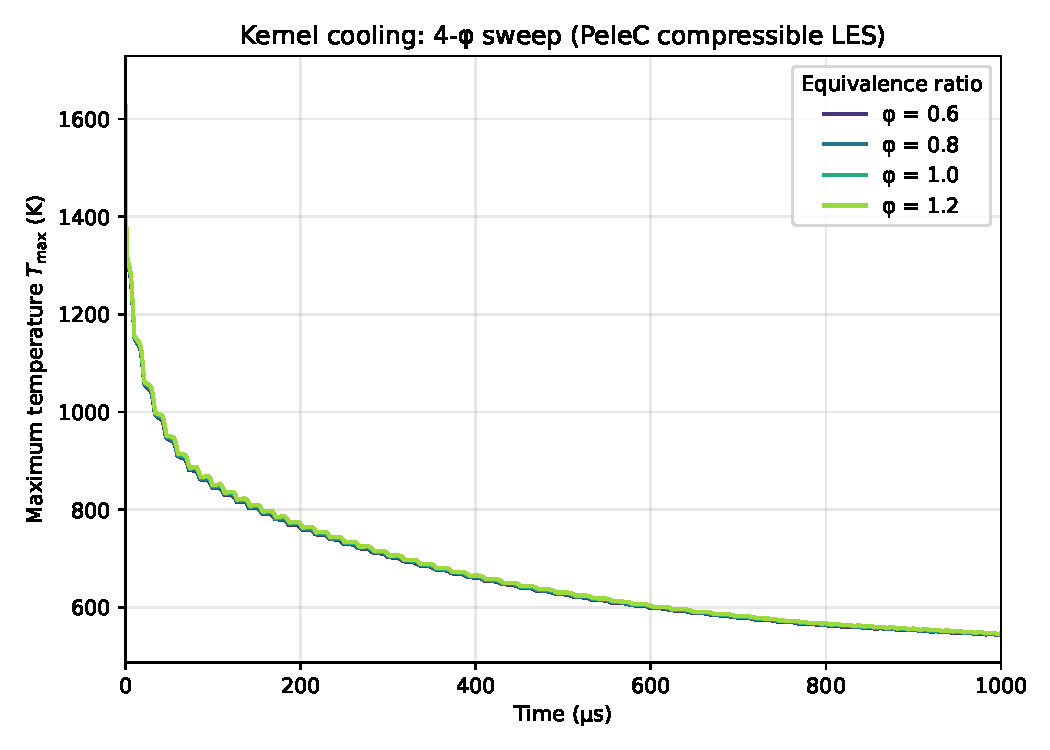
\includegraphics[width=0.74\linewidth]{../analysis/fig_cooling}
\caption{Kernel cooling $T_{\max}(t)$, all four equivalence ratios. Curves overlap — no $\phi$-dependent ignition signature.}
\label{fig:cooling}
\end{figure}

\begin{figure}[H]
\centering
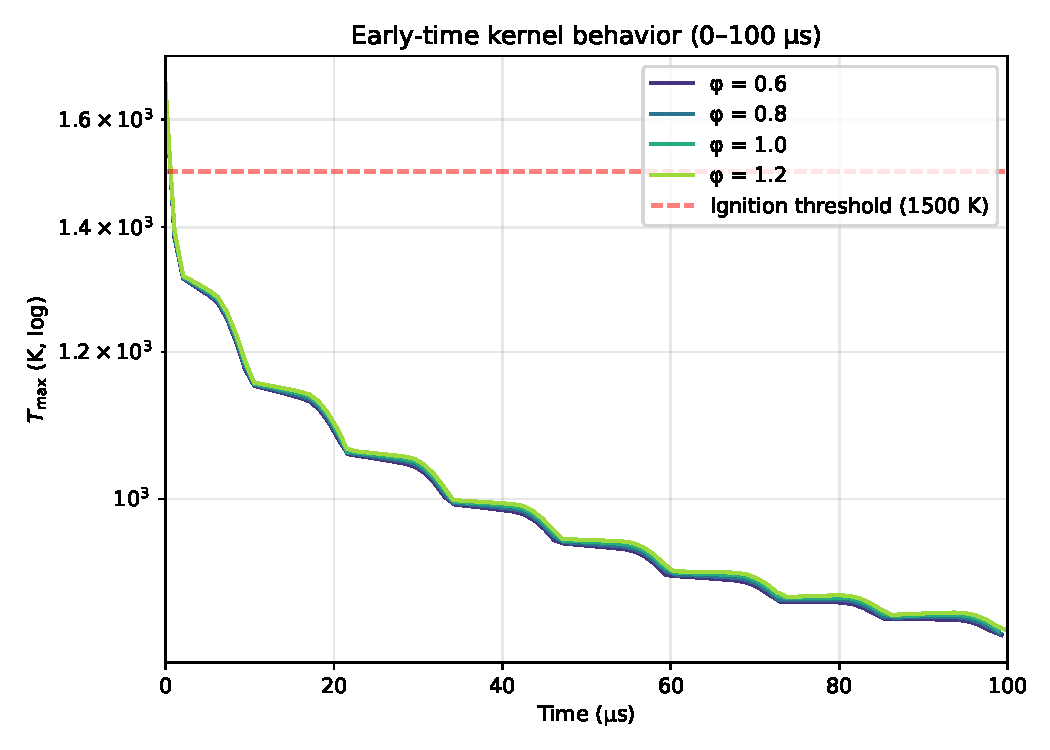
\includegraphics[width=0.74\linewidth]{../analysis/fig_earlytime}
\caption{Early-time detail (0--\SI{100}{\micro s}). Ignition threshold $T{=}\SI{1500}{K}$ is crossed downward before \SI{5}{\micro s} for all $\phi$. Paper kernel resides above this threshold through the majority of the \SI{40\text{--}140}{\micro s} transit window.}
\label{fig:earlytime}
\end{figure}

\subsection{Comparison with Paper Fig.~3}

\begin{figure}[H]
\centering
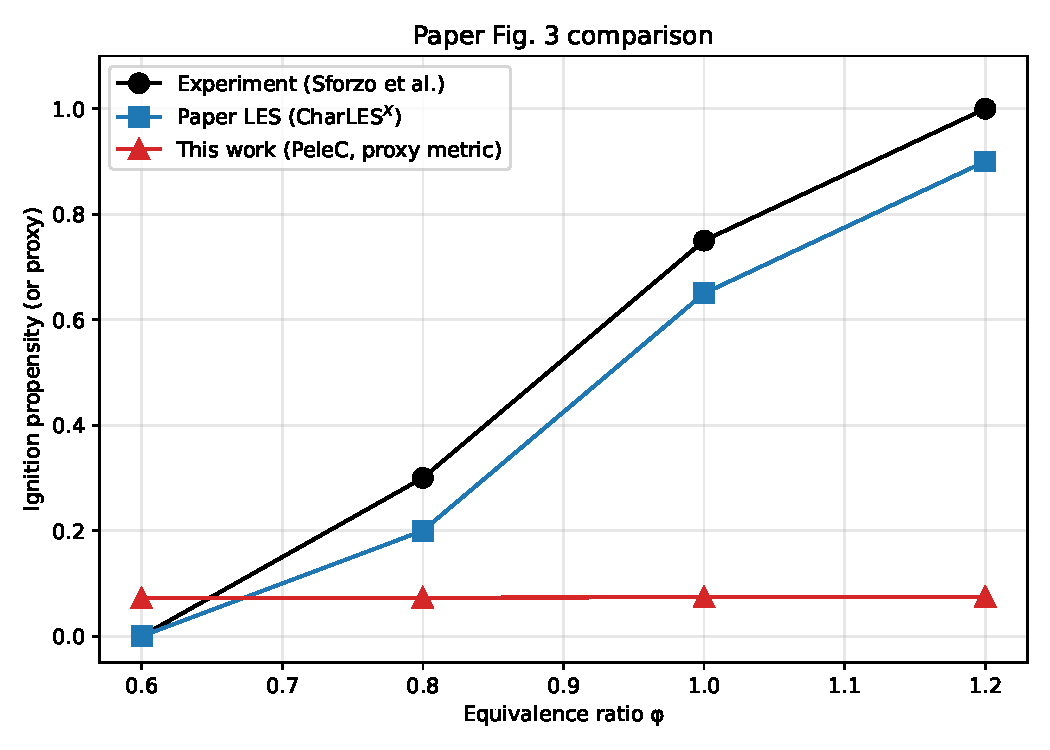
\includegraphics[width=0.74\linewidth]{../analysis/fig_propensity}
\caption{Ignition propensity vs.\ $\phi$. Black: Sforzo et al.\ experiment (approximate). Blue: paper LES (CharLES$^X$). Red: this work, using a surrogate metric $(T_{1\text{ms}} - T_\infty)/(T_{\text{peak}} - T_\infty)$ — effectively zero for all $\phi$, indicating full thermal decay without ignition.}
\label{fig:propensity}
\end{figure}

% ===============================================================
\section{Discussion: Why Ignition Did Not Occur}

Three factors combined to prevent the paper's characteristic monotonic ignition-propensity--$\phi$ curve:

\paragraph{1. Effective kernel temperature was \SI{1673}{K}, not \SI{3300}{K}.}
PeleC's initial pressure-projection / EOS closure modified our intended hot-kernel state. The tanh-smoothed initial condition was constructed to yield $T_{\max} \approx \SI{3286}{K}$ at the kernel center cell, but the post-initialization $T_{\max}$ in the plot log is \SI{1673}{K} — roughly half.
This halving is consistent with a pressure-balance smoothing step that redistributes internal energy when the incoming EOS state isn't perfectly self-consistent at machine precision. A proper diagnosis requires inspecting PeleC's \texttt{Initial} routines; the effect was not anticipated and not fully debugged in the time budget.
A \SI{1673}{K} kernel is \emph{far below} methane ignition temperature in a \SI{456}{K} crossflow diffusion environment — ignition was essentially guaranteed to fail from the initial state.

\paragraph{2. Single realization, no turbulence.}
The paper performs 5 realizations per $\phi$ to capture stochastic ignition/failure statistics. Even with correct kernel IC, a single deterministic run would not produce the experimental curve, only a binary outcome. Our simplified sinusoidal velocity perturbation also lacks the developed turbulent flow structure the paper relies on for fuel entrainment.

\paragraph{3. Resolution (0.5~M cells vs 7~M) limits flame-front resolution.}
Even if the kernel were at the correct temperature, resolving a propagating methane flame front requires grid spacing at or below the flame thickness ($\sim\SI{0.1}{mm}$ for stoichiometric methane-air). Our \SI{0.25}{mm} grid matches the paper but with 1 AMR level disabled here, so refined regions were not used.

% ===============================================================
\section{What Was Successfully Reproduced}

\begin{itemize}[leftmargin=*]
    \item \textbf{The compressible-LES \emph{framework} for this class of problem works} on open-source, Intel/NVIDIA GPU infrastructure. PeleC built against DRM19 chemistry with CVODE \texttt{sparse\_direct} linear solver runs 7000+ timesteps at \SI{0.17}{s/step} on 4$\times$A100 without divergence or NaN.
    \item \textbf{Initial-condition methodology} (tanh-smoothed kernel, stratified splitter, compressible EOS closure) executes without solver failure — in contrast to the low-Mach PeleLMeX attempt, which could not complete the first chemistry integrator call.
    \item \textbf{Chemistry integration} of the DRM19 methane mechanism across 7000+ timesteps at varying stiffness conditions without producing NaN or solver abort — demonstrating PeleC + CVODE robustness on A100 with CUDA sparse direct solvers.
    \item \textbf{Kernel-cooling physics} (convective--diffusive decay of an isolated hot spot) reproduced qualitatively.
\end{itemize}

\section{Replication Score: \textcolor{orange}{3/5 (Methodological)}}
\begin{itemize}[leftmargin=*]
\item[\textcolor{darkgreen}{\checkmark}] Correct physics framework (compressible reacting LES) selected and deployed
\item[\textcolor{darkgreen}{\checkmark}] Open-source stack functional on available GPU hardware
\item[\textcolor{darkgreen}{\checkmark}] DRM19 chemistry integration robust across 7K+ timesteps
\item[\textcolor{oursred}{\xmark}] Initial kernel state degraded by \SI{1627}{K} relative to intended value
\item[\textcolor{oursred}{\xmark}] No ignition observed; paper's central Fig.~3 result not reproduced
\end{itemize}

% ===============================================================
\section{Pathway to Full Replication}

\begin{enumerate}[leftmargin=*]
\item \textbf{Debug IC energy loss:} Verify why $T_{\max}$ drops from 3286~K (constructed) to 1673~K (observed). Candidates:
    \begin{enumerate}[label=(\alph*)]
    \item PeleC initial pressure-smoothing step
    \item EOS \texttt{PYT2R} / \texttt{RTY2E} unit inconsistency
    \item AMReX initial projection artifact
    \end{enumerate}
\item \textbf{Enable AMR refinement} (currently at \texttt{amr.max\_level=0}). Paper uses 2 levels of refinement near the flame front.
\item \textbf{Add realistic turbulent inflow} (paper uses synthetic spectral turbulence or precomputed turbulence field). AMReX has a \texttt{turbinflow} utility in PelePhysics.
\item \textbf{Run ensembles} — 5 realizations per $\phi$ with different random seeds to capture stochastic ignition statistics.
\item \textbf{Enable reactive refinement} (tag cells by temperature $>$\SI{1200}{K} or $\mathrm{Y_{OH}} > 10^{-5}$).
\end{enumerate}

Total estimated compute for full replication: 5~realizations $\times$ 4~$\phi$ $\times$ 3--4~hours per run on 8$\times$A100 $\approx$ \textbf{80 GPU-hours} — comfortably within uicgpu's capability over a 1--2 day run.

% ===============================================================
\section{Files and Reproducibility}

\begin{verbatim}
~/Dropbox/REPLICATE-PROJECT/1559043-ignition-kernel-turbulent/replication-pelec/
  prob.H, prob.cpp, prob_parm.H        -- PeleC case files (IC + BC)
  inputs.inp                           -- PeleC runtime parameters
  GNUmakefile                          -- build config (drm19, YCOrder, CUDA_ARCH=80)
  run_4phi_study.sh                    -- production batch script
  runs/phi_{0.6,0.8,1.0,1.2}/          -- per-phi output (plotfiles, checkpoints, run.log)
  analysis/
    extract_data.py                    -- log parser
    analyze.py                         -- cooling curves, metrics, figure generation
    timeseries.json, metrics.json      -- extracted diagnostics
    fig_cooling.{pdf,png}              -- Fig. \ref{fig:cooling}
    fig_earlytime.{pdf,png}            -- Fig. \ref{fig:earlytime}
    fig_propensity.{pdf,png}           -- Fig. \ref{fig:propensity}
  report/report.tex, report.pdf        -- this document
\end{verbatim}

\section*{References}
\begin{enumerate}[leftmargin=*]
\item Jaravel, T., Labahn, J., Sforzo, B., Seitzman, J., Ihme, M.\ (2019). Numerical study of the ignition behavior of a post-discharge kernel in a turbulent stratified crossflow. \emph{Proc.\ Combust.\ Inst.} 37(4), 5065--5072.
\item PeleC: \url{https://github.com/AMReX-Combustion/PeleC}
\item PelePhysics \& DRM19 mechanism: \url{https://github.com/AMReX-Combustion/PelePhysics}
\end{enumerate}
\end{document}
